\ifx\allfiles\undefined
\documentclass[12pt, a4paper,oneside, UTF8]{ctexbook}
\usepackage[dvipsnames]{xcolor}
\usepackage{mathtools}   % 数学公式(mathtools 是 amsmath 的上位替代)
\usepackage{amsthm}    % 定理环境
\usepackage{amssymb}   % 更多公式符号
\usepackage{graphicx}  % 插图
%\usepackage{mathrsfs}  % 数学字体
%\usepackage{newtxtext,newtxmath}
%\usepackage{arev}
\usepackage{kmath,kerkis}
\usepackage{newtxtext}
\usepackage{bbm}
\usepackage{enumitem}  % 列表
\usepackage{geometry}  % 页面调整
%\usepackage{unicode-math}
\usepackage[colorlinks,linkcolor=black]{hyperref}

\usepackage{wrapfig}


\usepackage{ulem}	   % 用于更多的下划线格式,
					   % \uline{}下划线,\uuline{}双下划线,\uwave{}下划波浪线,\sout{}中间删除线,\xout{}斜删除线
					   % \dashuline{}下划虚线,\dotuline{}文字底部加点


\graphicspath{ {flg/},{../flg/}, {config/}, {../config/} }  % 配置图形文件检索目录
\linespread{1.5} % 行高

% 页码设置
\geometry{top=25.4mm,bottom=25.4mm,left=20mm,right=20mm,headheight=2.17cm,headsep=4mm,footskip=12mm}

% 设置列表环境的上下间距
\setenumerate[1]{itemsep=5pt,partopsep=0pt,parsep=\parskip,topsep=5pt}
\setitemize[1]{itemsep=5pt,partopsep=0pt,parsep=\parskip,topsep=5pt}
\setdescription{itemsep=5pt,partopsep=0pt,parsep=\parskip,topsep=5pt}

% 定理环境
% ########## 定理环境 start ####################################
\theoremstyle{definition}
\newtheorem{defn}{\indent 定义}[section]

\newtheorem{lemma}{\indent 引理}[section]    % 引理 定理 推论 准则 共用一个编号计数
\newtheorem{thm}[lemma]{\indent 定理}
\newtheorem{corollary}[lemma]{\indent 推论}
\newtheorem{criterion}[lemma]{\indent 准则}

\newtheorem{proposition}{\indent 命题}[section]
\newtheorem{example}{\indent \color{SeaGreen}{例}}[section] % 绿色文字的 例 ,不需要就去除\color{SeaGreen}{}
\newtheorem*{rmk}{\indent \color{red}{注}}

% 两种方式定义中文的 证明 和 解 的环境:
% 缺点:\qedhere 命令将会失效【技术有限,暂时无法解决】
\renewenvironment{proof}{\par\textbf{证明.}\;}{\qed\par}
\newenvironment{solution}{\par{\textbf{解.}}\;}{\qed\par}

% 缺点:\bf 是过时命令,可以用 textb f等替代,但编译会有关于字体的警告,不过不影响使用【技术有限,暂时无法解决】
%\renewcommand{\proofname}{\indent\bf 证明}
%\newenvironment{solution}{\begin{proof}[\indent\bf 解]}{\end{proof}}
% ######### 定理环境 end  #####################################

% ↓↓↓↓↓↓↓↓↓↓↓↓↓↓↓↓↓ 以下是自定义的命令  ↓↓↓↓↓↓↓↓↓↓↓↓↓↓↓↓

% 用于调整表格的高度  使用 \hline\xrowht{25pt}
\newcommand{\xrowht}[2][0]{\addstackgap[.5\dimexpr#2\relax]{\vphantom{#1}}}

% 表格环境内长内容换行
\newcommand{\tabincell}[2]{\begin{tabular}{@{}#1@{}}#2\end{tabular}}

% 使用\linespread{1.5} 之后 cases 环境的行高也会改变,重新定义一个 ca 环境可以自动控制 cases 环境行高
\newenvironment{ca}[1][1]{\linespread{#1} \selectfont \begin{cases}}{\end{cases}}
% 和上面一样
\newenvironment{vx}[1][1]{\linespread{#1} \selectfont \begin{vmatrix}}{\end{vmatrix}}

\def\d{\textup{d}} % 直立体 d 用于微分符号 dx
\def\R{\mathbb{R}} % 实数域
\def\N{\mathbb{N}} % 自然数域
\def\C{\mathbb{C}} % 复数域
\def\Z{\mathbb{Z}} % 整数环
\def\Q{\mathbb{Q}} % 有理数域
\newcommand{\bs}[1]{\boldsymbol{#1}}    % 加粗,常用于向量
\newcommand{\ora}[1]{\overrightarrow{#1}} % 向量

% 数学 平行 符号
\newcommand{\pll}{\kern 0.56em/\kern -0.8em /\kern 0.56em}

% 用于空行\myspace{1} 表示空一行 填 2 表示空两行  
\newcommand{\myspace}[1]{\par\vspace{#1\baselineskip}}

%s.t. 用\st就能打出s.t.
\DeclareMathOperator{\st}{s.t.}

%罗马数字 \rmnum{}是小写罗马数字, \Rmnum{}是大写罗马数字
\makeatletter
\newcommand{\rmnum}[1]{\romannumeral #1}
\newcommand{\Rmnum}[1]{\expandafter@slowromancap\romannumeral #1@}
\makeatother
\begin{document}
	% \title{{\Huge{\textbf{$Partial \,\, Differential \,\, Equations$}}}\footnote{参考书籍:\\
			\hspace*{4em} \textbf{《Partial Differential Equations》 -- Lawrence C. Evans} \\
			\hspace*{4em} \textbf{《Partial Differential Equations》 -- Fritz John} \\
			\hspace*{4em} \textbf{《数学物理方程讲义 (第二版)》--  姜礼尚、陈亚浙、刘西垣、易法槐} 
			}}
\author{$-TW-$}
\date{\today}
\maketitle                   % 在单独的标题页上生成一个标题

\thispagestyle{empty}        % 前言页面不使用页码
\begin{center}
	\Huge\textbf{序}
\end{center}


\vspace*{3em}
\begin{center}
	\large{\textbf{天道几何,万品流形先自守;}}\\
	
	\large{\textbf{变分无限,孤心测度有同伦。}}
\end{center}

\vspace*{3em}
\begin{flushright}
	\begin{tabular}{c}
		\today \\ \small{\textbf{长夜伴浪破晓梦,梦晓破浪伴夜长}}
	\end{tabular}
\end{flushright}


\newpage                      % 新的一页
\pagestyle{plain}             % 设置页眉和页脚的排版方式(plain:页眉是空的,页脚只包含一个居中的页码)
\setcounter{page}{1}          % 重新定义页码从第一页开始
\pagenumbering{Roman}         % 使用大写的罗马数字作为页码
\tableofcontents              % 生成目录

\newpage                      % 以下是正文
\pagestyle{plain}
\setcounter{page}{1}          % 使用阿拉伯数字作为页码
\pagenumbering{arabic}
\setcounter{chapter}{0}    % 设置 -1 可作为第零章绪论从第零章开始 
	\else
	\fi
	%  ############################ 正文部分
\appendix
\chapter{Supplementary Content}\label{appendix A}

\section{变分原理与最小曲面问题}
	所谓\textbf{变分问题}, 即\textbf{求某一特定泛函在定义域内的极值}. 下面要介绍的\textbf{最小曲面问题}即为一个典型的变分问题.  
	
\subsection{Cut-Off Function}
	先来回顾数分中给出过最常见的\textbf{Cut-Off Function (截断函数)}. 下面以2维情况为例. 
	
	\begin{example}\label{ex A.1.1}
		Define 
		\begin{align*}
			\rho(x , y) = 
			\begin{cases}
				k \, e^{-\tfrac{1}{1 - (x^2 + y^2)}} , \,\, x^2 + y^2 < 1 \\
				0 , \,\, x^2 + y^2 \geq 1
			\end{cases}
		\end{align*}
		Then $\rho \in C_{0}^{\infty} (\R^2)$. We can choose $k \in \R$, $\st$
		\begin{align*}
			\iint_{\R^2} \rho(x , y) \, dx dy = 1
		\end{align*}
		Fix the taken $k \in \R$. 为了方便缩小紧支集的范围, 我们进一步定义
		\begin{align*}
			\rho_{n}(x , y) = n^2 \rho(nx , ny) , \,\, \forall n \in \N
		\end{align*}
		Then $\rho_n \in C^{\infty}_0 (\R^2)$ and $\rho_{n}(x , y) \equiv 0 , \,\, \forall \sqrt{x^2 + y^2} \geq \dfrac{1}{n}$.
		\begin{align*}
			\iint_{\R^2} \rho_{n}(x , y) \, dxdy = 1 , \,\, \forall n \in \N
		\end{align*}
	\end{example}
	
	\vspace*{4em}
	
	下面利用\textbf{Cut-Off Function}, 给出一条引理, 在证明\textbf{最小曲面问题的等价问题}时会用到. 
	
	\newpage
	
	此处给出n维的一般性结论. 
	
	\begin{lemma}\label{lemma A.1.1}
		Suppose $\Omega \subset \R^n$ be open and bounded, $f \in C(\Omega)$. If $\forall \varphi \in C_{0}^{\infty} (\Omega)$, we have 
		\begin{align*}
			\int_{\Omega} f(x) \varphi(x) \, dx = 0
		\end{align*}
		Then $f \equiv 0$ on $\Omega$. 
		
		\vspace*{8em}
		
		\begin{proof}
			反证法. Assume $\exists x_0 \in \Omega$, $\st f(x_0) \neq 0$. 不妨设$f(x_0) > 0$. \\
			Since $f \in C(\Omega)$, $\Omega \subset \R^n$ open, then $\exists \delta > 0$, $\st$
			\[ f(x) > 0 , \,\, \forall x \in B_{\delta}(x_0) \subset \Omega \]
			Fix $\delta > 0$. Take $N \in \N$ satisfies $\dfrac{1}{N} \leq \delta$. Let
			\[ \varphi(x) = \rho_{N}(x - x_0) , \,\, \forall x \in \R^n \]
			Then $\varphi \in C_{0}^{\infty}(\Omega)$ and
			\begin{align*}
				\int_{\Omega} f(x) \varphi(x) \, dx 
				= \int_{B_{\delta}(x_0)} f(x) \rho_{N}(x - x_0) \, dx 
				> 0
			\end{align*}
			which contradicts to $\iint_{\Omega} f(x) \varphi(x) \, dx = 0 , \,\, \forall \varphi \in C_{0}^{\infty} (\Omega)$. \\
			Therefore, $f \equiv 0$ on $\Omega$. 
		\end{proof}
	\end{lemma}

\newpage

\subsection{极小曲面问题}
	考虑$\R^2$ 上有界区域$\Omega \subset \R^2$.  \textbf{极小曲面问题}即指给定边界$\partial \Omega$ 上一条闭曲线l:
	\begin{align*}
		l : 
		\begin{cases}
			x = x(s) \\
			y = y(s) \\
			u = \varphi(s)
		\end{cases} , \,\, 0 \leq s \leq s_0
	\end{align*}
	其中$x = x(s) , y = y(s)$ 为平面曲线$\partial \Omega$ 的方程. 求一张定义在$\overline{\Omega}$ 上的曲面$S$, $\st$
	\begin{center}
		$S$ 以$l$ 为边界, 且表面积最小. 
	\end{center}
	我们定义
	\begin{align*}
		M_{\varphi} = \Big\{ v \in C^1(\overline{\Omega}) \,\, \Big| \,\, v |_{\partial \Omega} = \varphi \Big\}
	\end{align*}
	上述问题即可表示为下述\textbf{变分问题}:
	\begin{align*}
		u = \underset{v \in M_{\varphi}}{\text{argmin}} \,\, J(v)
	\end{align*}
	where
	\begin{align*}
		J : M_{\varphi} &\longrightarrow \R \\
		v &\longmapsto J(v) = \iint_{\Omega} \sqrt{1 + v_{x}^2 + v_{y}^2} \, dxdy
	\end{align*}
	
	\vspace*{4em}
	
	下面我们直接给出\textbf{极小曲面问题}的解的\textbf{必要条件 (需满足的方程)}, 事实上我们将说明, 当要求解满足一定光滑性时 ($C^2(\Omega) \cap C^1(\overline{\Omega})$), 这个条件为\textbf{充要条件}. 
	
	\newpage
	
	\begin{thm}\label{thm A.1.2}
		\textbf{[Minimal Surface]}. \\
		Suppose $\Omega \subset \R^2$ be a bounded region, $\partial \Omega \in C^{\infty}$, $\varphi \in C^1(\partial \Omega)$. Suppose $u \in C^2(\Omega) \cap C^1(\overline{\Omega})$ satisfies 
		\[ u \Big|_{\partial \Omega} = \varphi \]
		Let
		\[ M_{\varphi} = \Big\{ v \in C^1(\overline{\Omega}) \,\, \Big| \,\, v \big|_{\partial \Omega} = \varphi \Big\} \]
		Then 
		\begin{center}
			$u = \underset{v \in M_{\varphi}}{\text{argmin}} \,\, J(v) \,\, \Longleftrightarrow \,\, (1 + u_{y}^2) u_{xx} - 2 u_{x} u_{y} \cdot u_{xy} + (1 + u_{x}^2) u_{yy} = 0$
		\end{center}
		where
		\[ J(v) = \iint_{\Omega} \sqrt{1 + v_{x}^2 + v_{y}^2} \, dxdy , \,\, \forall v \in M_{\varphi} \]
			
		\vspace*{6em}
		
		\begin{rmk}
			若没有\textbf{“$u \in C^2(\Omega)$”}的光滑性条件, 则结论中的\textbf{“$\Leftrightarrow$”} 应当换为\textbf{“$\Rightarrow$”}, 即
			\begin{center}
				$(1 + u_{y}^2) u_{xx} - 2 u_{x} u_{y} \cdot u_{xy} + (1 + u_{x}^2) u_{yy} = 0$
			\end{center}
			是$u$ 为极小曲面问题的解的\textbf{必要条件}. 
		\end{rmk}
		
		\vspace*{6em}
		
		\begin{proof}
			\begin{itemize}
				\item \textbf{必要性“$\Rightarrow$”}:Suppose $u = \underset{v \in M_{\varphi}}{\text{argmin}} \,\, J(v)$. 记
				\[ M_0 = \Big\{ v \in C^1(\overline{\Omega}) \,\, \Big| \,\, v \big|_{\partial \Omega} = 0 \Big\} \]
				Then for $\forall v \in M_0$, we have $u + \epsilon v \in M_{\varphi} , \,\, \forall \epsilon \in \R$. Let
				\begin{align*}
					j : \R &\longrightarrow \R \\
					\epsilon &\longmapsto j(\epsilon) = J(u + \epsilon v)
				\end{align*}
				Then
				\begin{align*}
					j^{'}(\epsilon) 
					&=  \iint_{\Omega} \frac{\partial}{\partial \epsilon} \sqrt{1 + (u_x + \epsilon v_x)^2 + (u_y + \epsilon v_y)^2} \, dxdy \\
					&= \iint_{\Omega} \frac{v_x (u_x + \epsilon v_x) + v_y (u_y + \epsilon v_y)}{\sqrt{1 + (u_x + \epsilon v_x)^2 + (u_y + \epsilon v_y)^2}} \, dxdy
				\end{align*}
				Since $u = \underset{v \in M_{\varphi}}{\text{argmin}} \,\, J(v)$, then $j(\epsilon)$ achieves its minimum at $\epsilon = 0$. Thus
				\[ j^{'}(0) = 0 \]
				i.e.
				\begin{align*}
					\iint_{\Omega} \Big( \frac{u_x}{\sqrt{1 + u_{x}^2 + u_{y}^2}} v_x + \frac{u_y}{\sqrt{1 + u_{x}^2 + u_{y}^2}} v_y \Big) \, dxdy = 0 , \,\, \forall v \in M_{0}
				\end{align*}
				Let $\nabla f\footnote{此处$f$的存在性并未证明, 待修正.} = \Big( \dfrac{u_x}{\sqrt{1 + u_{x}^2 + u_{y}^2}} , \dfrac{u_y}{\sqrt{1 + u_{x}^2 + u_{y}^2}} \Big)$, then by \textbf{第一Green恒等式}, 
				\begin{align*}
					\iint_{\Omega} \nabla f \cdot \nabla v \, dxdy 
					= -\iint_{\Omega} \Delta f \, v \, dxdy + \int_{\partial \Omega} \frac{\partial f}{\partial \gamma} v \, dS
				\end{align*}
				Since $v \in M_{0}$, $v \equiv 0$ on $\partial \Omega$, then 
				\begin{align*}
					\iint_{\Omega} \left\{ \frac{\partial}{\partial x} \Big[ \frac{u_x}{\sqrt{1 + u_{x}^2 + u_{y}^2}} \Big] + \frac{\partial}{\partial y} \Big[ \frac{u_y}{\sqrt{1 + u_{x}^2 + u_{y}^2}} \Big] \right\} v \, dxdy = 0 , \,\, \forall v \in M_0
				\end{align*}
				Since $C_{0}^{\infty}(\Omega) \subset M_0$, then by \textbf{Lemma \ref{lemma A.1.1}}, 
				\begin{align*}
					\frac{\partial}{\partial x} \Big[ \frac{u_x}{\sqrt{1 + u_{x}^2 + u_{y}^2}} \Big] + \frac{\partial}{\partial y} \Big[ \frac{u_y}{\sqrt{1 + u_{x}^2 + u_{y}^2}} \Big] \equiv 0 \,\, \text{on} \,\, \Omega
				\end{align*}
				i.e.
				\begin{align*}
					(1 + u_{y}^2) u_{xx} - 2 u_{x} u_{y} \cdot u_{xy} + (1 + u_{x}^2) u_{yy} = 0
				\end{align*}
				
				\newpage
				
				\item \textbf{充分性“$\Leftarrow$”}:Suppose $u \in C^2(\Omega) \cap C^1(\overline{\Omega})$ satisfies 
				\begin{align*}
					(1 + u_{y}^2) u_{xx} - 2 u_{x} u_{y} \cdot u_{xy} + (1 + u_{x}^2) u_{yy} = 0
				\end{align*}
				i.e.
				\begin{align*}
					\frac{\partial}{\partial x} \Big[ \frac{u_x}{\sqrt{1 + u_{x}^2 + u_{y}^2}} \Big] + \frac{\partial}{\partial y} \Big[ \frac{u_y}{\sqrt{1 + u_{x}^2 + u_{y}^2}} \Big] \equiv 0 \,\, \text{on} \,\, \Omega
				\end{align*}
				Let 
				\[ M_0 = \Big\{ v \in C^2(\Omega) \cap C^1(\overline{\Omega}) \,\, \Big| \,\, v \big|_{\partial \Omega} = 0 \Big\} \]
				By \textbf{Green第一恒等式 (Thm \ref{cor B.4.3})}, 倒着必要性的证明过程, 不难得到
				\[ j^{'}(0) = 0 , \,\, \forall v \in M_0 \]
				Since $u , v \in C^2(\Omega) \cap C^1(\overline{\Omega})$, then calculate
				\begin{align*}
					j^{''}(\epsilon) 
					= \iint_{\Omega} \frac{v_{x}^2 + v_{y}^2 + \Big[ v_y (u_x + \epsilon v_x)_x - v_{x} (u_y + \epsilon v_y)_y \Big]^2}{\Big[ \sqrt{1 + (u_x + \epsilon v_x)^2 + (u_y + \epsilon v_y)^2} \Big]^3} dxdy > 0 , \,\, \forall \epsilon \in \R
				\end{align*}
				又因为$j^{'}(0) = 0$, Therefore, 
				\[ u = \underset{v \in M_{\varphi}}{\text{argmin}} \,\, J(v) \]
			\end{itemize}
		\end{proof}
	\end{thm}

\newpage

\section{线性PDE的叠加原理}

	\begin{thm}\label{thm A.2.1}
		\textbf{[线性PDE的叠加原理]}. \\
		Suppose $L$ be a linear partial differential operator, $\{ u_i \}_{i = 1}^{\infty}$ be the solutions of these equations respectively 
		\[ Lu = f_{i} , \,\, i = 1 , 2 , \cdots \]
		若$u_i$ 存在2阶偏导数, 且级数$\overset{\infty}{\underset{i = 1}{\sum}} {c_i u_i} , \,\, \overset{\infty}{\underset{i = 1}{\sum}} {c_i f_i}$ 均收敛, 记$u = \overset{\infty}{\underset{i = 1}{\sum}} {c_i u_i}$. 则$u$ 为方程
		\[ Lu = \sum_{i = 1}^{\infty} {c_i f_i} \]
		的解. 
		
		\vspace*{2em}
		
		\begin{rmk}
			事实上该命题是Trivial的, 即对于\textbf{线性微分算子$L$}, 其对于任意有限项求和线性. 再根据级数的收敛性可知, $L$ 对于可数项求和线性. 
		\end{rmk}
	\end{thm}

\newpage

\section{一维波动方程的Duhamel原理 (齐次化原理)}
	对于\textbf{一维波动方程}的初值问题
	\begin{align*}
		\begin{cases}
			\dfrac{\partial^2 u}{\partial t^2} - c^2 \dfrac{\partial^2 u}{\partial x^2} = f(x , t) , \,\, x \in \R , t > 0 \\
			u \Big|_{t = 0} = \varphi(x) \\
			u_t \Big|_{t = 0} = \psi(x)
		\end{cases}
	\end{align*}
	根据\textbf{线性PDE的叠加原理(Thm \ref{thm A.2.1})}, 其解可以表示为
	\[ u = u_1 + u_2 + u_3 \]
	其中$u_1 , u_2 , u_3$ 分别为下述三个初值问题的解:
	
	\vspace*{1em}
	
	\begin{align}
		&\begin{cases}
			\dfrac{\partial^2 u_1}{\partial t^2} - c^2 \dfrac{\partial^2 u_1}{\partial x^2} = 0 , \,\, x \in \R , t > 0 \\
			u_1 \Big|_{t = 0} = \varphi(x) \\
			u_{1_t} \Big|_{t = 0} = 0
		\end{cases} \\ 
		&\begin{cases}
			\dfrac{\partial^2 u_2}{\partial t^2} - c^2 \dfrac{\partial^2 u_2}{\partial x^2} = 0 , \,\, x \in \R , t > 0 \\
			u_2 \Big|_{t = 0} = 0 \\
			u_{2_t} \Big|_{t = 0} = \psi(x)
		\end{cases}\label{A.2} \\
		&\begin{cases}
			\dfrac{\partial^2 u_3}{\partial t^2} - c^2 \dfrac{\partial^2 u_3}{\partial x^2} = f(x , t) , \,\, x \in \R , t > 0 \\
			u_3 \Big|_{t = 0} = 0 \\
			u_{3_t} \Big|_{t = 0} = 0
		\end{cases}
	\end{align}
	
	\vspace*{4em}
	
	下面我们说明, 对于$u_1$ 与$u_3$, 其可由$u_2$ 表出, 这就是\textbf{Duhamel原理 (齐次化原理)}. 
	
	\newpage
	
	\begin{thm}\label{thm A.3.1}
		\textbf{[一维波动方程的Duhamel原理 (齐次化原理)]\footnote{详细证明可参考书籍:\textbf{《数学物理方程讲义 (第二版)》--  姜礼尚、陈亚浙、刘西垣、易法槐} -- $\S 2.2$ 定理 2.1 .}}. \\
		设$u_2 = M_{\psi}(x , t)$ 为定解问题(\ref{A.2}) 的解, 此处$M_\psi$ 表示以$\psi$ 为初值的定解问题(\ref{A.2}) 的解, 则$u_1$ 和$u_3$ 可表示为
		\begin{align*}
			\begin{cases}
				u_1 = \dfrac{\partial}{\partial t} M_{\varphi}(x , t) \\
				u_3 = \int_{0}^t M_{f_{\tau}} (x , t - \tau) \, d\tau
			\end{cases}
		\end{align*}
		where $f_{\tau} = f(x , \tau)$.
	\end{thm}

\newpage

\section{一维波动方程的能量不等式}
	\begin{thm}\label{thm A.4.1}
		\textbf{[一维波动方程的能量不等式]}. \\
		记上半平面$Q = \R \times (0 , \infty)$. 设$u \in C^1(\overline{Q}) \cap C^2(Q)$ 为定解问题(\ref{2.10}) 的解, 即
		\begin{align*}
			\begin{cases}
				\dfrac{\partial^2 u}{\partial t^2} - c^2 \dfrac{\partial^2 u}{\partial x^2} = f(x , t) , \,\, x \in \R , t > 0 \\
				u \Big|_{t = 0} = \varphi(x) \\
				u_t \Big|_{t = 0} = \psi(x)
			\end{cases}
		\end{align*}
		则对于$M = e^{t_0} > 0$, $\forall (x_0 , t_0) \in \R \times (0 , \infty)$, $\st$
		\begin{align}
			\int_{\Omega_\tau} [ u_{t}^2 + c^2 u_{x}^2 ] 
			\leq M \left[ \int_{\Omega_0} ( \psi^2 + c^2 \varphi_{x}^2 ) + \iint_{K_\tau} f^2 \right] , \,\, \forall \tau \in [0 , t_0] 
		\end{align}
		
		\begin{align}
			\iint_{K_\tau} [u_{t}^2 + c^2 u_{x}^2] 
			\leq M \left[ \int_{\Omega_0} (\psi^2 + c^2 \varphi_{x}^2) + \iint_{K\tau} f^2 \right] , \,\, \forall \tau \in [0 , t_0]
		\end{align}
		
		\vspace*{1em}
		
		\hspace*{-1.85em}其中有关区域$K_{\tau}$ 定义如下 (与\textbf{Thm \ref{thm 2.3.1}} 中保持一致)
		
		\begin{figure}[thbp!]
			\centering
			\begin{minipage}[t]{0.59\linewidth}
				\centering
				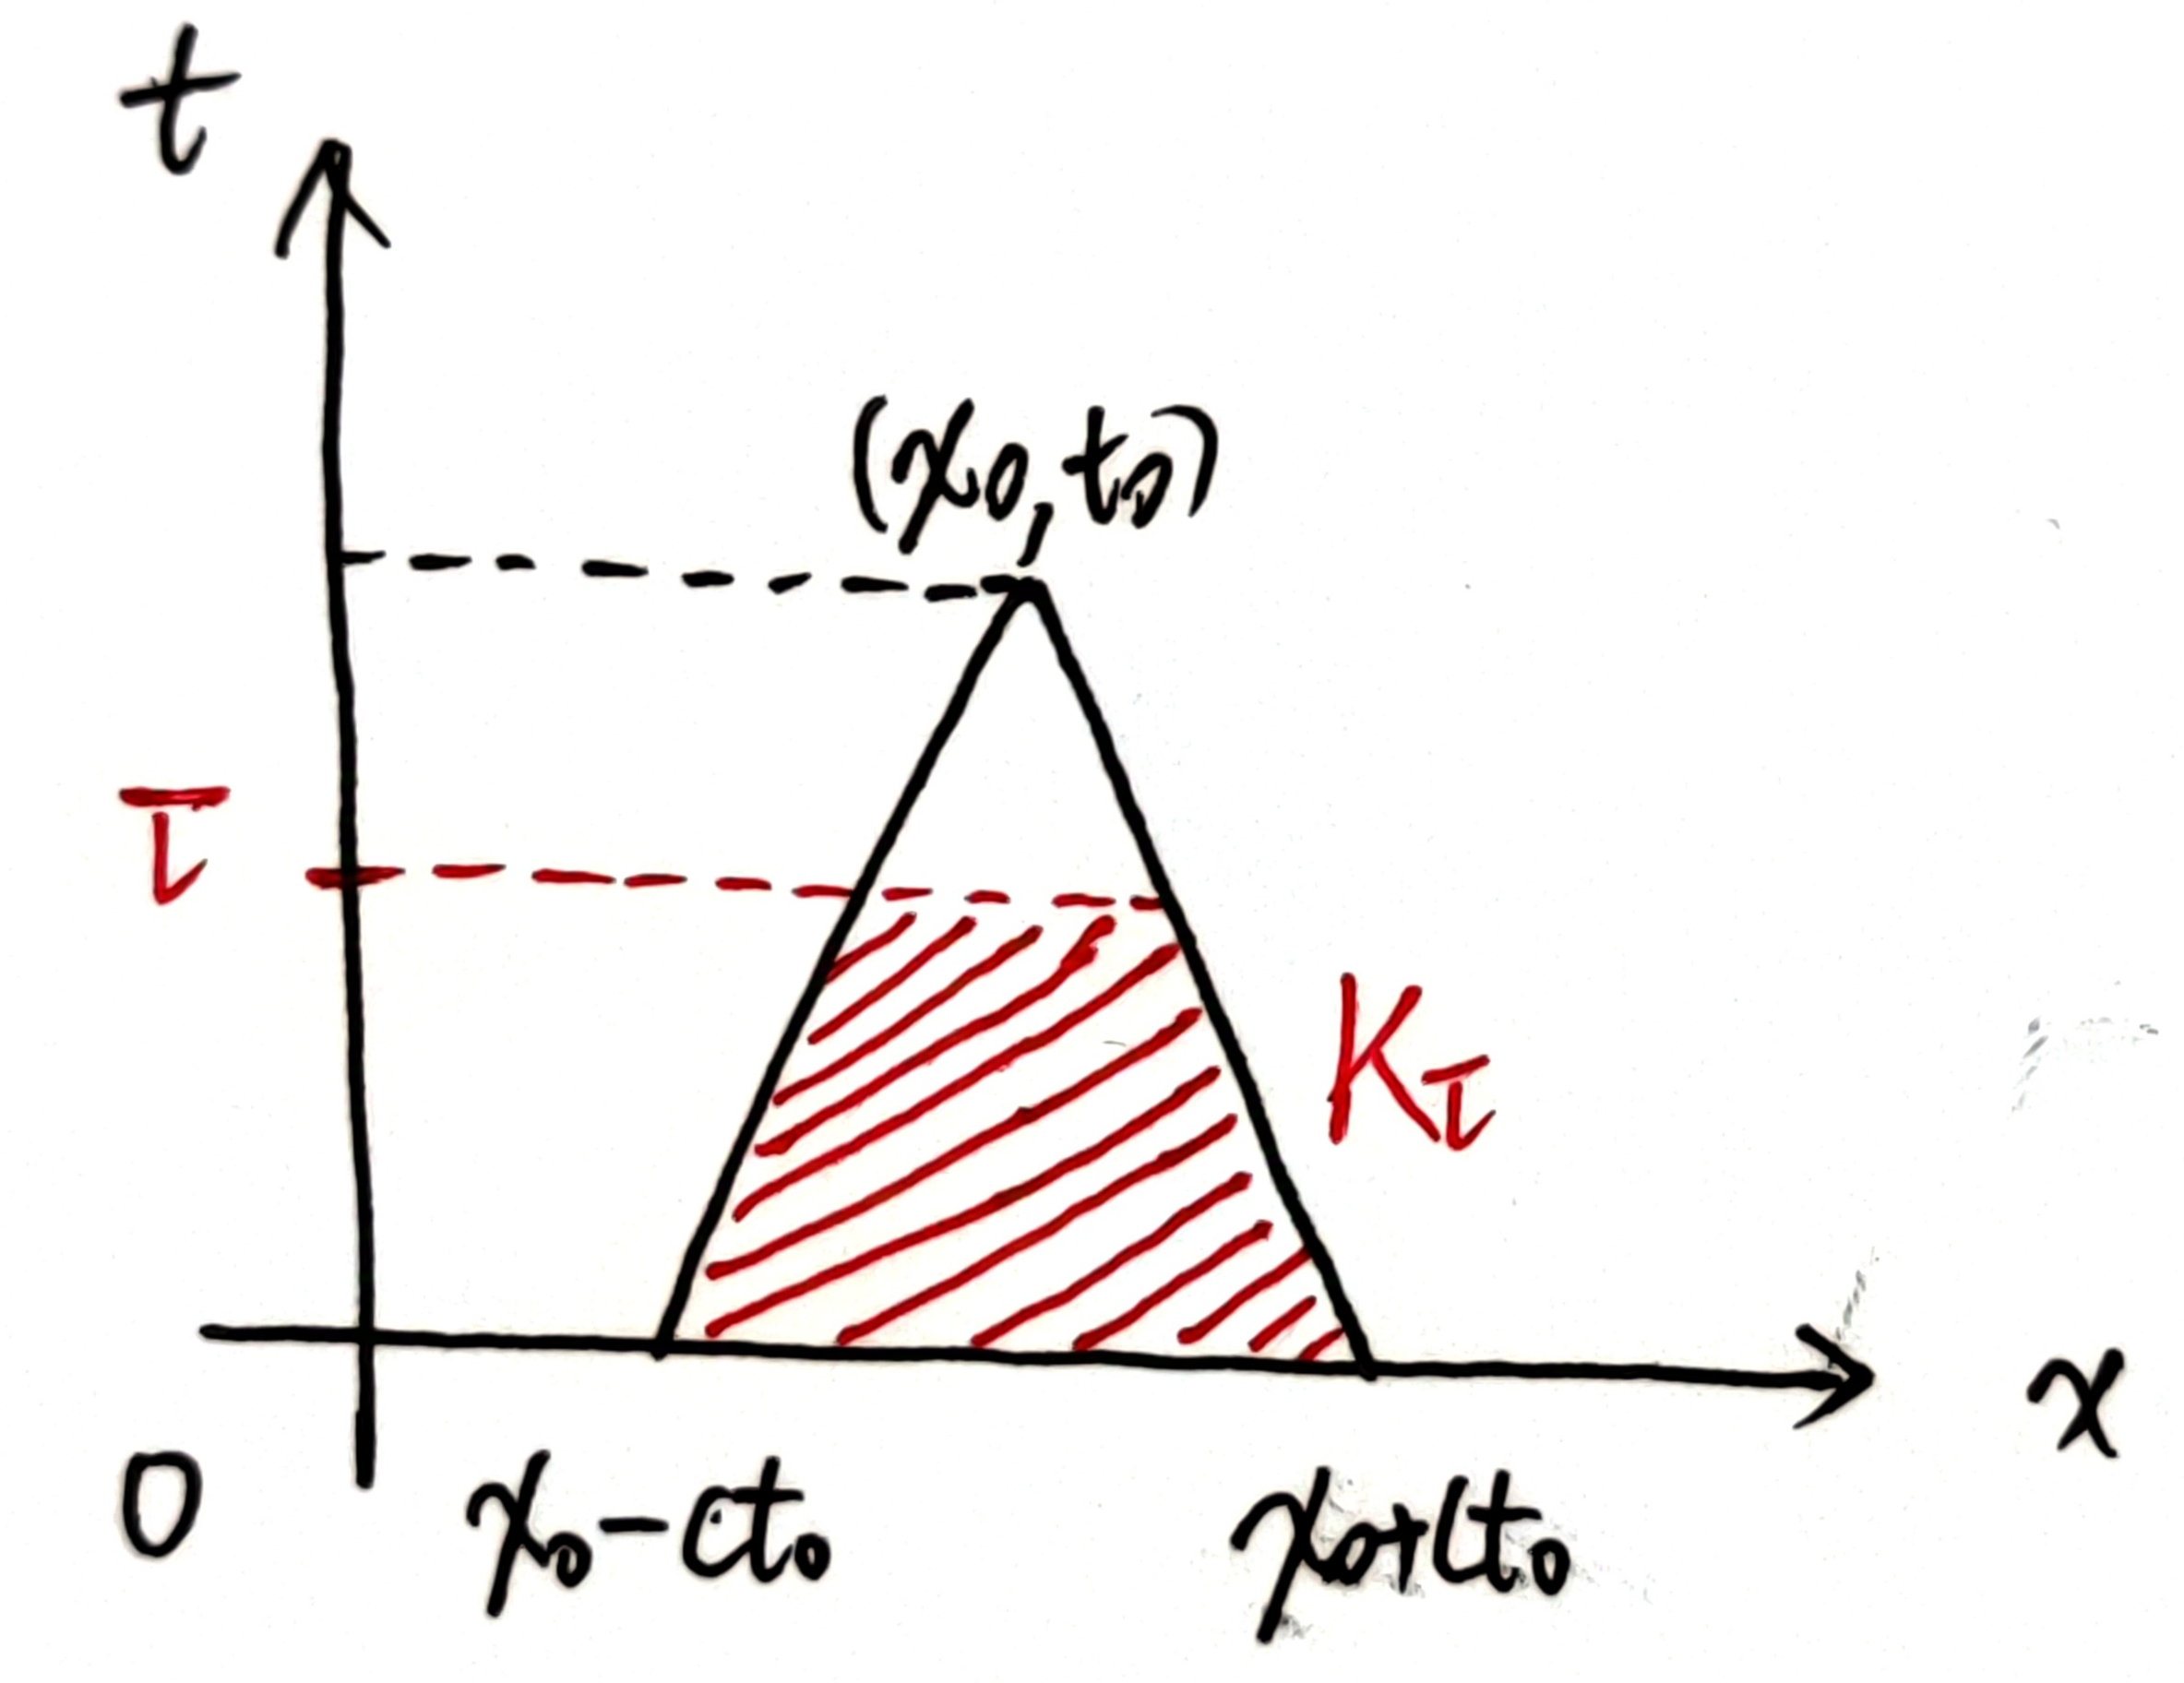
\includegraphics[width=0.65\linewidth]{figure/2.3-4}
				\caption{依赖区间及区域$K_\tau$ 的定义}
				\label{fig : A.4-1}
			\end{minipage}
			\begin{minipage}[t]{0.39\linewidth}
				\centering
				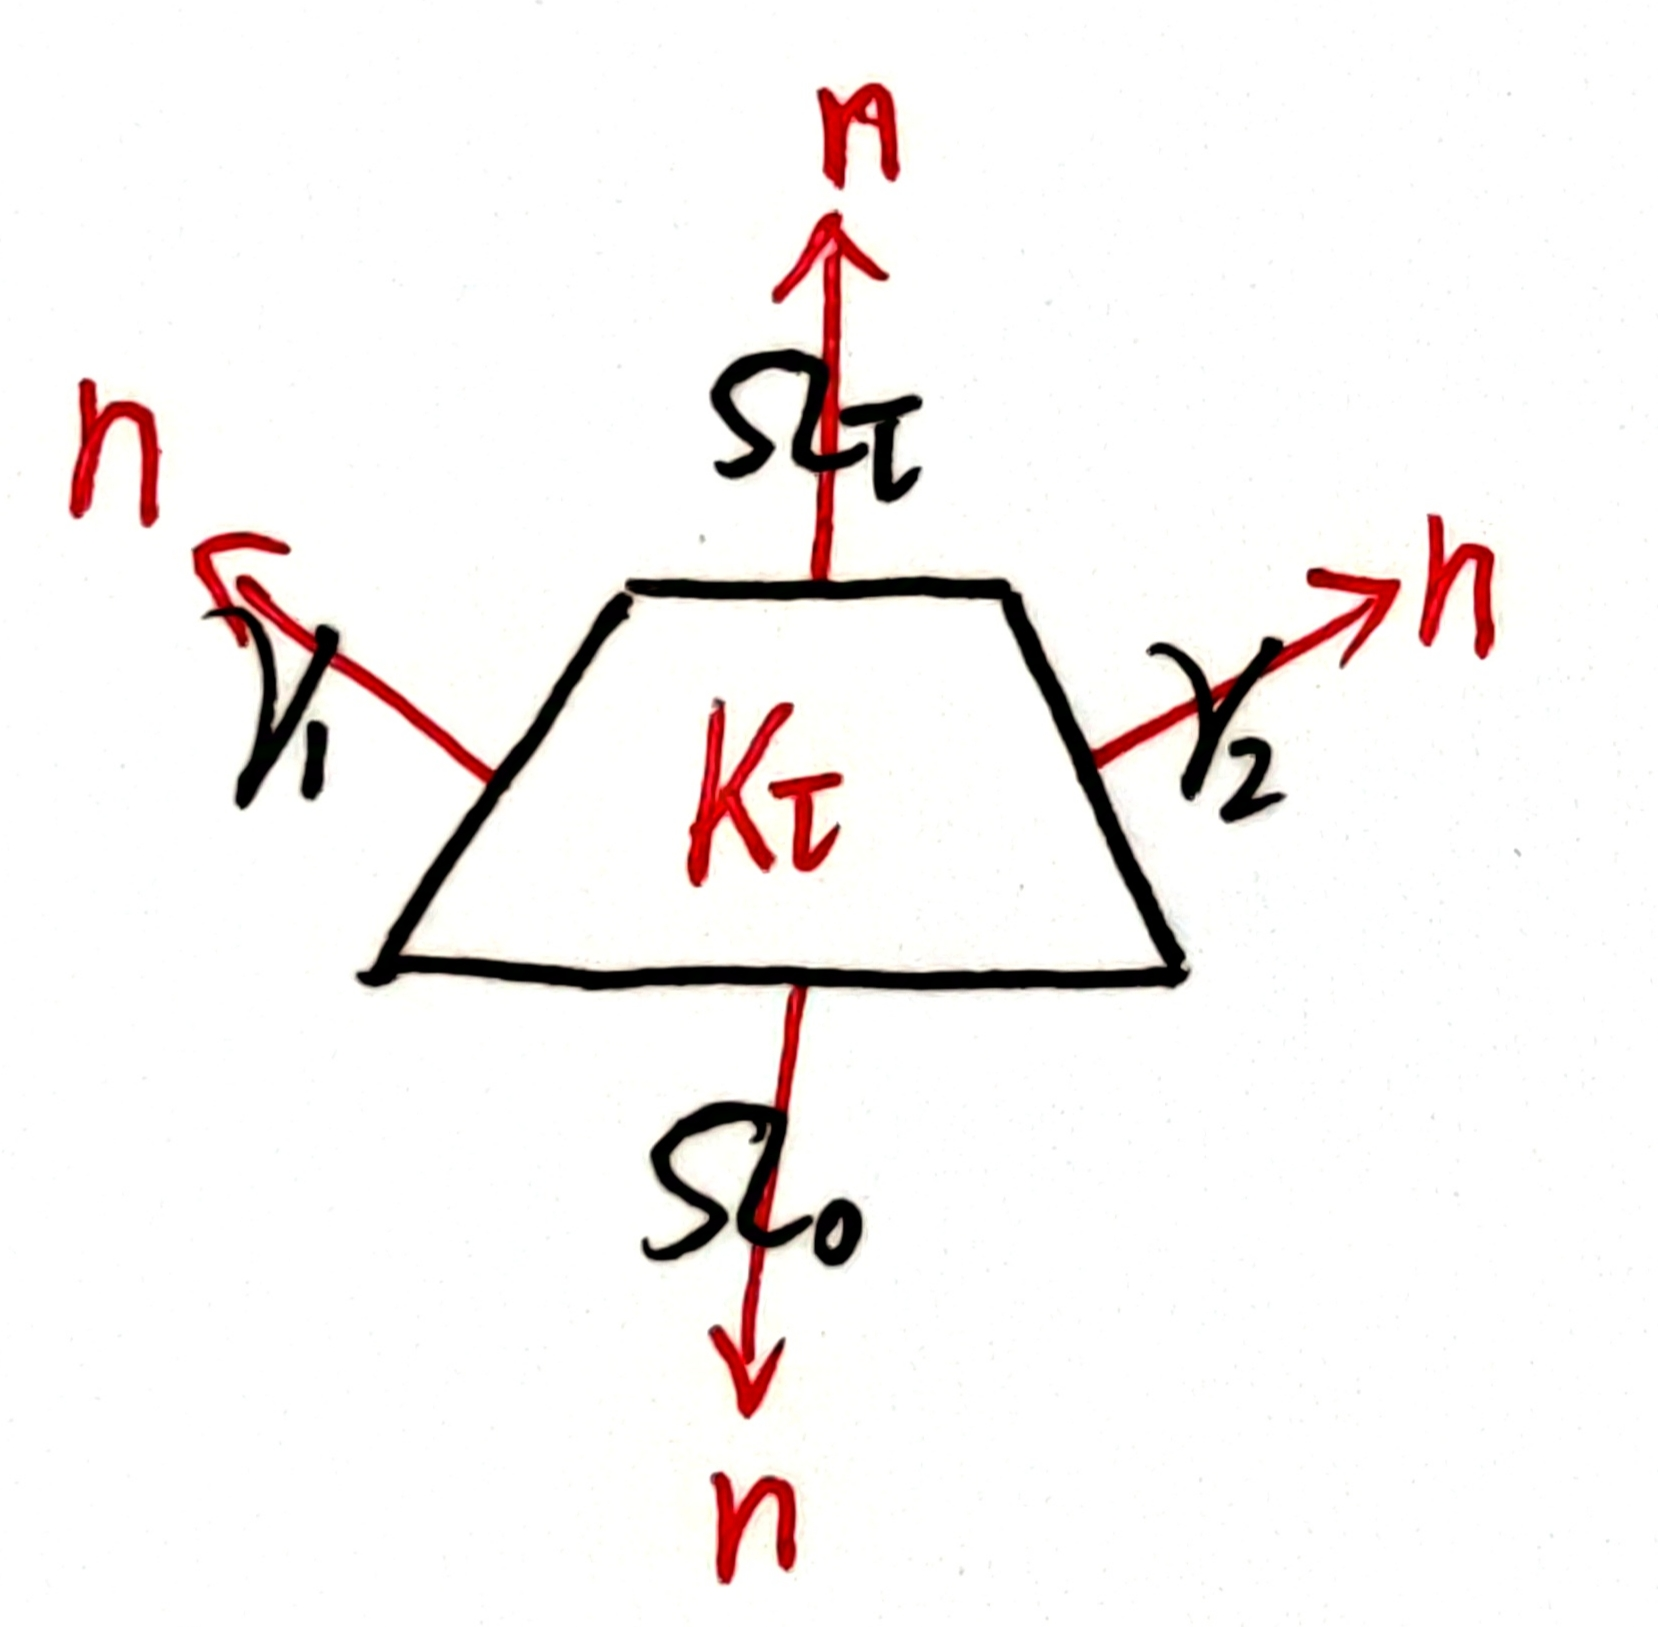
\includegraphics[width=0.55\linewidth]{figure/2.3-5}
				\caption{区域$K_\tau$ 各边记号及法向}
				\label{fig : A.4-2}
			\end{minipage}
		\end{figure}
	\end{thm}
	
	\newpage
	
	在证明\textbf{能量不等式 (Thm \ref{thm A.4.1})} 之前, 先给出一个引理. 
	
	\begin{lemma}\label{lemma A.4.2}
		\textbf{[Gronwall Inequality]}. \\
		设非负函数$G \in C[0 , T]$, $G(\tau) \geq 0$. 若$G(0) = 0$, 且对于$\forall \tau \in [0 , T]$, $\st$
		\[ \frac{dG(\tau)}{d \tau} \leq C \cdot G(\tau) + F(\tau) \,\, \text{for some} \,\, C > 0 \]
		where $F(\tau)$ 为$[0 , T]$ 上递增的非负可积函数, 则有
		\begin{align*}
			\frac{dG(\tau)}{d\tau} &\leq e^{C\tau} F(\tau) , \,\, \forall \tau \in [0 , T] \\
			G(\tau) &\leq \frac{e^{C\tau} - 1}{C} F(\tau) , \,\, \forall \tau \in [0 , T]
		\end{align*}
		
		\vspace*{8em}
		
		\begin{proof}
			Since $\dfrac{dG(\tau)}{d \tau} \leq C \cdot G(\tau) + F(\tau)$, then 等式两侧同乘$e^{-C\tau}$, we have
			\[ \frac{d}{d\tau} \Big[ e^{-C\tau} G(\tau) \Big] \leq e^{-C\tau} F(\tau) , \,\, \forall \tau \in [0 , T] \]
			等式两边在$[0 , \tau]$ 上积分, since $F(\tau)$ 在$[0 , T]$ 上递增非负, then
			\[ e^{-C\tau} G(\tau) \leq \int_{0}^\tau e^{-Ct} F(t) \, dt \leq F(\tau) \cdot \frac{1 - e^{-C\tau}}{C} , \,\, \forall \tau \in [0 , T] \]
			i.e.
			\[ G(\tau) \leq \frac{e^{C\tau} - 1}{C} F(\tau) , \,\, \forall \tau \in [0 , T] \]
			将上述不等式代入$\dfrac{dG(\tau)}{d \tau} \leq C \cdot G(\tau) + F(\tau)$ 右侧, 即可得到
			\[ \frac{dG(\tau)}{d\tau} \leq e^{C\tau} F(\tau) , \,\, \forall \tau \in [0 , T] \]
		\end{proof}
	\end{lemma}
	
	\newpage
	
	\begin{proof}
		下面开始证明\underline{\textbf{能量不等式}}:\\
		Since $u_{tt} - c^2 u_{xx} = f(x , t)$ on $\R \times (0 , \infty)$, then
		\[ \iint_{K_\tau} u_t(u_{tt} - c^2 u_{xx}) = \iint_{K_\tau} u_t \cdot f \]
		对于等式左边, 与\textbf{Thm \ref{thm 2.3.1}-唯一性} 证明过程一致 (\ref{2.13}), 利用\textbf{Gauss-Green 公式 (Thm \ref{thm B.4.1})}, 可得到
		\[ \int_{\Omega_\tau} [ u_{t}^2 + c^2 u_{x}^2 ] \leq \int_{\Omega_0} [ \psi^2 + c^2 \varphi_{x}^2 ] + 2\iint_{K_\tau} u_t \cdot f \]
		根据均值不等式$2ab \leq a^2 + b^2 , \,\, \forall a , b \in \R$, then
		\[ \int_{\Omega_\tau} [ u_{t}^2 + c^2 u_{x}^2 ] \leq \int_{\Omega_0} [ \psi^2 + c^2 \varphi_{x}^2 ] + \iint_{K_\tau} u_{t}^2 + \iint_{K_\tau} f^2 \]
		Let
		\[ G(\tau) = \iint_{K_\tau} [u_{t}^2 + c^2 u_{x}^2] = \int_{0}^\tau \Big( \int_{\Omega_t} [ u_{t}^2 + c^2 u_{x}^2 ] \, dx \Big) \, dt \]
		Then $G \in C[0 , t_0]$, $G \geq 0$, $G(0) = 0$. 且对于$\forall \tau \in [0 , t_0]$, $\st$
		\begin{align*}
			\frac{dG(\tau)}{d\tau} = \int_{\Omega_0} [u_{t}^2 + c^2 u_{x}^2] 
			\leq \iint_{K\tau} u_{t}^2 + F(\tau) 
			\leq G(\tau) + F(\tau)
		\end{align*}
		i.e.
		\[ \frac{dG(\tau)}{d\tau} \leq G(\tau) + F(\tau) , \,\, \forall \tau \in [0 , t_0] \]
		where 
		\[ F(\tau) = \int_{\Omega_0} [\psi^2 + c^2 \varphi_{x}^2] + \iint_{K_\tau} f^2 \geq 0 \,\, \text{在$[0 , t_0]$ 上非负递增可积} \]
		Thus by \textbf{Gronwall Inequality (Lemma \ref{lemma A.4.2})}, for $C = 1$, 
		\begin{align*}
			\frac{dG(\tau)}{d\tau} &\leq e^{\tau} F(\tau) \leq e^{t_0} F(\tau) , \,\, \forall \tau \in [0 , t_0] \\
			G(\tau) &\leq ( e^{\tau} - 1 ) F(\tau) \leq e^{t_0} F(\tau) , \,\, \forall \tau \in [0 , t_0]
		\end{align*}
		i.e.
		\begin{align*}
			\int_{\Omega_\tau} [u_{t}^2 + c^2 u_{x}^2] 
			\leq M \left[ \int_{\Omega_0} ( \psi^2 + c^2 \varphi_{x}^2 ) + \iint_{K_\tau} f^2 \right] , \,\, \forall \tau \in [0 , t_0] 
		\end{align*}
		and
		\begin{align*}
			\iint_{K_\tau} [u_{t}^2 + c^2 u_{x}^2] 
			\leq M \left[ \int_{\Omega_0} (\psi^2 + c^2 \varphi_{x}^2) + \iint_{K\tau} f^2 \right] , \,\, \forall \tau \in [0 , t_0]
		\end{align*}
		where $M = e^{t_0} > 0$. 
	\end{proof}








\chapter{Fundamental Knowledge}\label{appendix B}

\section{区域边界的光滑性}
	下面我们来给出\textbf{区域边界的光滑性}的定义.

	\begin{defn}\label{def B.1.1}
		Suppose $\Omega \subset \R^n$ is open, $\partial \Omega \neq \varnothing$. 如果对于$\forall p \in \partial \Omega$, $\exists p$ 的邻域$U$, $\st$ 在适当的空间直角坐标系下, 
		\begin{align}
			\partial \Omega \cap U &= \{ (x^{'} , x^{n}) \in \R^{n - 1} \times \R \mid x^{'} \in D , \,\, x^n = \varphi(x^{'}) \} \\
			\Omega \cap U &= \{ (x^{'} , x^n) \in \R^{n - 1} \times \R \mid x^{'} \in D , \,\, x^n > \varphi(x^{'}) 	\} \cap U
		\end{align}
		where $\varphi \in C^{k}(\Omega) , \,\, D \subset \R^{n - 1}$ open. 我们称\underline{\textcolor{blue}{\textbf{$\partial \Omega \in C^k$}}}, 这里$k = 0 , 1 , 2 , \cdots$ 或$\infty$.
	
		\begin{figure}[thbp!]
			\centering
			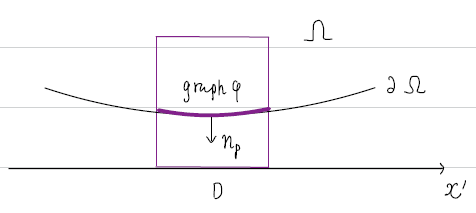
\includegraphics[width=0.5\linewidth]{figure/A.1-1}
			\caption{边界的光滑性}
			\label{pic : A.1-1} % 添加图像引用标签
		\end{figure}
	
		\begin{rmk}
			在\textbf{定义 \ref{def B.1.1}} 中, 设$k \leq 1$, $\,\, x_{0}^{'} \in \partial \Omega$, $\,\, p = (x_{0}^{'} , \varphi(x_{0}^{'}))$. 记
			\[ n_p = \frac{(\nabla \varphi(x_{0}^{'}) , -1)}{\sqrt{1 + \left| \nabla \varphi(x_{0}^{'}) \right|^2}} \]
			称$n_p$ 为$\partial \Omega$ 在$p$ 点的\underline{\textcolor{blue}{\textbf{单位外法向}}}. $n_p$ 的定义与空间直角坐标系的选择无关. 记
			\begin{align}
				n : \partial \Omega &\longrightarrow \R^n \\
				p &\longmapsto n(p) = n_p 
			\end{align}
			称$n$ 为$\partial \Omega$ 的\underline{\textcolor{blue}{\textbf{单位外法向}}}. 因为$\partial \Omega \in C^k$, $k \geq 1$, 所以$n \in C(\partial \Omega ; \R^n)$.
		\end{rmk}
	\end{defn}

\newpage

\section{ODE解的存在唯一性定理}
	\begin{thm}\label{thm B.2.1}
		\textbf{[ODE解的存在唯一性]}.
	\end{thm}
	
	\begin{figure}[thbp!]
		\centering
		\includegraphics[width=1.1\linewidth]{figure/B.2-1}
		\caption{ODE解的存在唯一性}
		\label{pic : B.2-1} % 添加图像引用标签
	\end{figure}

\newpage

\section{反函数定理}
	\begin{thm}\label{thm B.3.1}
		\textbf{[反函数定理]}. \\
		Suppose $f \in C^{1}(\Omega ; \R^n)$, $\Omega \subset \R^n$ open, $x_0 \in \Omega$. If $Df|_{x_0}$ 可逆, then $\exists x_0$ 的邻域$U \subset \Omega$, $\st$ \\
		$f(U) \subset \R^n$ open, and
		\[ f : U \longrightarrow f(U) \,\, \textbf{为$C^1$-微分同胚} \]
	\end{thm}

\newpage

\section{Gauss-Green公式}
	首先回顾一下\textbf{外法向向量}及\textbf{(外)法向方向导数}的记号.
	\begin{itemize}
		\item Suppose $U \subset \R^n$. If $\partial U \in C^1$, then along $\partial U$ is defined the outward pointing unit normal vector field.\footnote{关于区域边界光滑性$\partial \Omega \in C^k$ 即\textbf{单位外法向}的定义, 详见\textbf{附录 \ref{appendix B}-定义 \ref{def B.1.1}}}
		\[ \vec{\gamma} = (\gamma^1 , \gamma^2 , \cdots , \gamma^n) 
		\hspace*{2em} , \hspace*{2em} 
		\vec{\gamma}(x^0) = \gamma = (\gamma_1 , \gamma_2 , \cdots , \gamma_n) \]
	
		\begin{rmk}
			我们总是将向量值函数的分量写作上标, 在具体某点的取值 (一般向量)写作下标.
		\end{rmk}
	
		\vspace{2em}
	
		\item Let $u \in C^{1}(\overline{U})$. We call $\,\, \dfrac{\partial u}{\partial \gamma} \coloneqq \vec{\gamma} \cdot Du \,\,$ the (outward) normal derivative of $u$.
	\end{itemize}

	\vspace{6em}

	下面我们给出多元微积分中十分重要的\textbf{Gauss-Green公式}, 又称\textbf{散度定理}.

	\begin{thm}\label{thm B.4.1}
		\textbf{[Gauss-Green Theorem]}. \\
		Suppose $U \subset \R^n$ is open and bounded, $\partial U \in C^1$.
		\begin{enumerate}
			\item[(\rmnum{1})] If $u \in C^{1}(\overline{U})$, then
			\begin{align}
				\int_{U} u_{x_i} = \int_{\partial U} u \gamma^i , \,\, \forall 1 \leq i \leq n
			\end{align}
		
			\item[(\rmnum{2})] $\forall$ vector field $\vec{u} \in C^{1}(\overline{U} ; \R^n)$,
			\begin{align}
				\int_{U} div \, \vec{u} = \int_{\partial U} \vec{u} \cdot \vec{\gamma}
			\end{align}
		\end{enumerate}
	
		\vspace{2em}
	
		\begin{rmk}
			\begin{itemize}
				\item (\rmnum{2})即为\textbf{Gauss-Green公式 (Gauss公式)}, 说明了对于$\R^n$ 中任一有界区域$U$ 	中的向量场$\vec{u}$, 其散度$div \, \vec{u}$ 在整个区域上的积分 = 其在整个边界$\partial U$ 上的通量.
			
				\vspace{1em}
			
				而散度作为描述向量场中某个点\textbf{向外发散程度}的标量, 原式可理解为:
				\begin{center}
					向量场$\vec{u}$ 在区域$U$ 中每个点发散程度的积累, 经过内部每个点散度相互抵消后, 最终等于其在边界$\partial 	U$ 处向外通量的总和.
				\end{center}
			
				\newpage
			
				\item \textbf{Gauss公式}事实上为\textbf{Green公式}在$n$ 维空间上的推广, 即\textbf{Green公式}事实上给出了二维空间$\R^2$ 上的\textbf{散度定理}. 在(\rmnum{2})中, 取$\vec{u} = (P , Q)$, 外法向方向为$\vec{\gamma} = (-dy , dx)$, 有:
				\[ \int_{U} \frac{\partial P}{\partial x} + \frac{\partial Q}{\partial y} 
				= \int_{\partial U} -P dy + Q dx \]
				简单地交换$P , Q$ 顺序即可得到最常见的\textbf{Green公式}的格式.
			
				\vspace{6em}
			
				\item 定理中(\rmnum{1})可作为(\rmnum{2})的直接推论. 即可令$\vec{u}$ 中除第$i$ 个分量$u^i$ 外均为0, 即$\vec{u} = (0 , \cdots , u^i , \cdots , 0)$, then
				\[ \int_{U} \frac{\partial u^i}{\partial x_i} = \int_{\partial U} u^i \gamma^i \]
				令$u = u^i \in C^{1}(\overline{U})$, 即可得到
				\[ \int_{U} u_{x_i} = \int_{\partial U} u \gamma^i , \,\, \forall 1 \leq i \leq n \]
			\end{itemize}
		\end{rmk}
	\end{thm}

	\vspace{11em}

	下面给出一系列根据\textbf{Gauss-Green公式}得到的推论, 在$PDE$ 中经常使用. 首先是所谓的\textbf{分部积分公式}.

	\begin{corollary}\label{cor B.4.2}
		\textbf{[Integration by parts formula]}. \\
			Let $u , v \in C^{1}(\overline{U})$, then
		\begin{align}
			\int_{U} u_{x_i} v = -\int_{U} u v_{x_i} + \int_{\partial U} u v \gamma^i
		\end{align}
	
		\vspace{6em}
	
		\begin{proof}
			在\textbf{Gauss-Green公式 (Thm \ref{thm B.4.1} (\rmnum{1}))}中, 将$u$ 换成$uv$, 即可得到
			\[ \int_{U} (u_{x_i}v + u v_{x_i}) = \int_{\partial U} u v \gamma^i \]
		\end{proof}
	\end{corollary}

	\newpage

	最后再给出三条常用的\textbf{Green恒等式}, 这也是\textbf{Gauss-Green公式}的直接推论.

	\begin{corollary}\label{cor B.4.3}
		\textbf{[Green's Formula]}. \\
		Let $u , v \in C^{2}(\overline{U})$, then
		\begin{enumerate}
			\item[(\rmnum{1})]
			\begin{align}
				\int_{U} \Delta u = \int_{\partial U} \frac{\partial u}{\partial \gamma}
			\end{align}
		
			\item[(\rmnum{2})]
			\begin{align}
				\int_{U} Du \cdot Dv = -\int_{U} u \Delta v + \int_{\partial U} u \frac{\partial v}{\partial \gamma} \hspace*{2em} \text{(\textbf{Green第一恒等式})}
			\end{align}
		
			\item[(\rmnum{3})]
			\begin{align}
				\int_{U} (u \Delta v - v \Delta u) = \int_{\partial U} \left( u \frac{\partial v}{\partial \gamma} - v \frac{\partial u}{\partial \gamma} \right) \hspace*{2em} \text{(\textbf{Green第二恒等式})}
			\end{align}
		\end{enumerate}
	
		\vspace{6em}
	
		\begin{proof}
			\begin{enumerate}
				\item[(\rmnum{1})] 将\textbf{Gauss-Green公式 (Thm \ref{thm B.4.1} (\rmnum{2}))} 中的$u$ 换为$\nabla u$, 得
				\[ \int_{U} \Delta u = \int_{\partial U} \nabla u \cdot \vec{\gamma} = \int_{\partial U} \frac{\partial u}{\partial \gamma} \]
			
				\vspace{2em}
			
				\item[(\rmnum{2})] 将\textbf{Gauss-Green公式 (Thm \ref{thm B.4.1} (\rmnum{2}))} 中的$u$ 换为$u \nabla v$, 由于
				\[ div(u \nabla v) = u \Delta v + \nabla u \cdot \nabla v = u \Delta v + Du \cdot Dv \]
				因此有
				\[ \int_{U} (u \Delta v + Du \cdot Dv) 
				= \int_{\partial U} u \nabla v \cdot \vec{\gamma} 
				= \int_{\partial U} u \frac{\partial v}{\partial \gamma} \]
			
				\vspace{2em}
			
				\item[(\rmnum{3})] 由于(\rmnum{2}) 中左式$u , v$ 对称, 因此交换$u , v$ 位置, 可得
				\begin{align}
					\int_{U} Du \cdot Dv &= -\int_{U} u \Delta v + \int_{\partial U} u \frac{\partial v}{\partial \gamma} \\
					\int_{U} Du \cdot Dv &= -\int_{U} v \Delta u + \int_{\partial U} v \frac{\partial u}{\partial \gamma}
				\end{align}
				两式相减即可得证.
			\end{enumerate}
		\end{proof}
	\end{corollary}

\newpage

\section{一阶常系数线性ODE的求解}
	
	\begin{thm}\label{thm B.5.1}
		\textbf{[一阶常系数线性ODE]}. \\
		对于一阶常系数线性ODE
		\begin{align*}
			\frac{d^n x}{dt^n} + a_1 \frac{d^{n - 1} x}{d t^{n - 1}} + \cdots + a_{n - 1} \frac{dx}{dt} + a_n x = 0
		\end{align*}
		其特征方程为
		\begin{align*}
			\lambda^n + a_1 \lambda^{n - 1} + \cdots + a_{n - 1} \lambda + a_n = 0
		\end{align*}
		对应的特征根 (可相等)为$\lambda_1 , \cdots , \lambda_n$. 则方程的通解可写为如下基本解组的线性组合:
		
		\vspace*{1em}
		
		\begin{enumerate}
			\item[(a)] 对每个单重实根$\lambda_k$ 有解$e^{\lambda_k t}$. 
			
			\vspace*{1em}
			
			\item[(b)] 对每个$m > 1$ 重实根$\lambda_k$ 有$m$ 个解
			\[ e^{\lambda_k t} , \,\, te^{\lambda_k t} , \cdots , \,\, t^{m - 1} e^{\lambda_k t} \]
			
			\vspace*{1em}
			
			\item[(c)] 对每一对重数为1的共轭复根$\alpha \pm i \beta$, 有2个如下形式的解
			\[ e^{\alpha t} \cos \beta t , e^{\alpha t} \sin \beta t \]
			
			\vspace*{1em}
			
			\item[(d)] 对每一对$m > 1$ 重共轭复根$\alpha \pm i \beta$, 有$2m$ 个如下形式的解
			\begin{align*}
				&e^{\alpha t} \cos \beta t , \,\, t e^{\alpha t} \cos \beta t , \cdots , \,\, t^{m - 1} e^{\alpha t} \cos \beta t \\
				&e^{\alpha t} \sin \beta t , \,\, t e^{\alpha t} \sin \beta t , \cdots , \,\, t^{m - 1} e^{\alpha t} \sin \beta t
			\end{align*}
		\end{enumerate}
	\end{thm}






	%  ############################
	\ifx\allfiles\undefined
\end{document}
\fi